

\section{Station de recharge}
\label{s:Recharge}

\begin{figure}[htp]
   \centering
   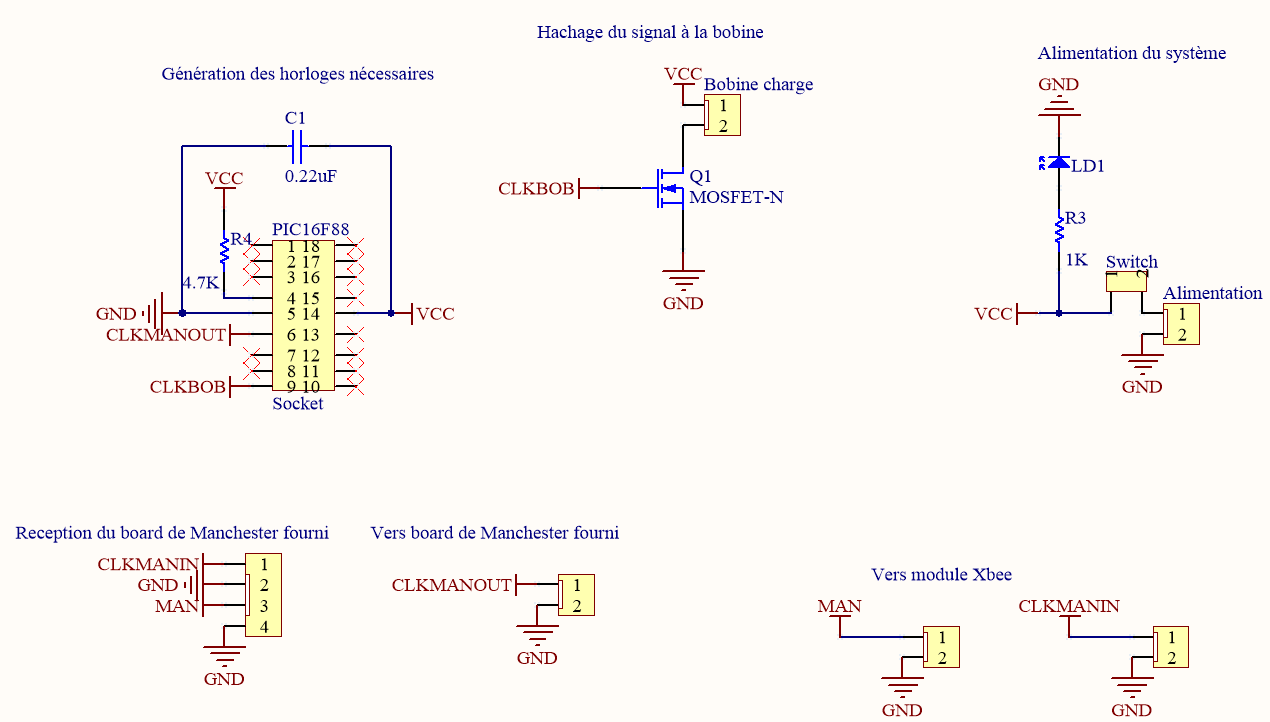
\includegraphics[width=1\textwidth]{fig/StationRecharge.png}
   \caption{Sch�ma �lectrique de la station de recharge}
   \label{f:StationRecharge}
\end{figure}


\section{Circuit d'amplification du code Manchester}
\label{s:Manchester}

\begin{figure}[htp]
   \centering
   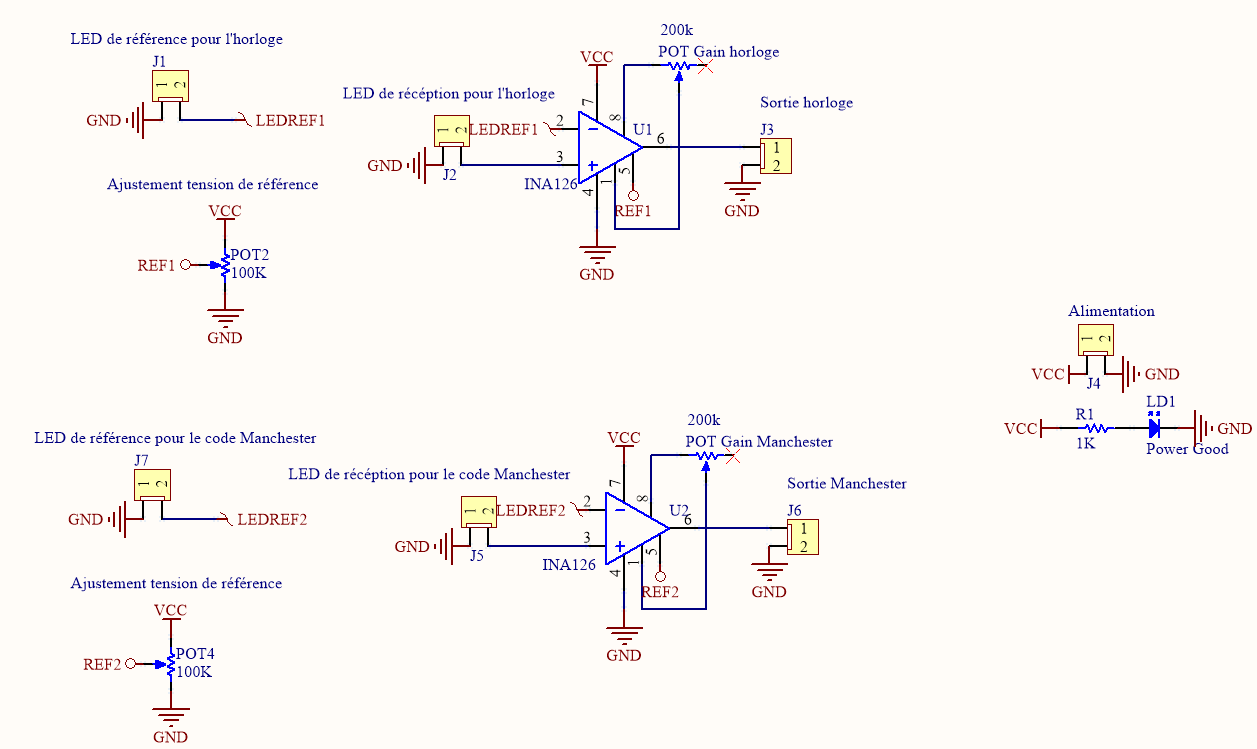
\includegraphics[width=1\textwidth]{fig/Manchester.png}
   \caption{Sch�ma �lectrique du circuit d'amplification du code Manchester}
   \label{f:Manchester}
\end{figure}


\section{Circuit de charge et de d�charge du condensateur}
\label{s:Condensateur}

\begin{figure}[htp]
   \centering
   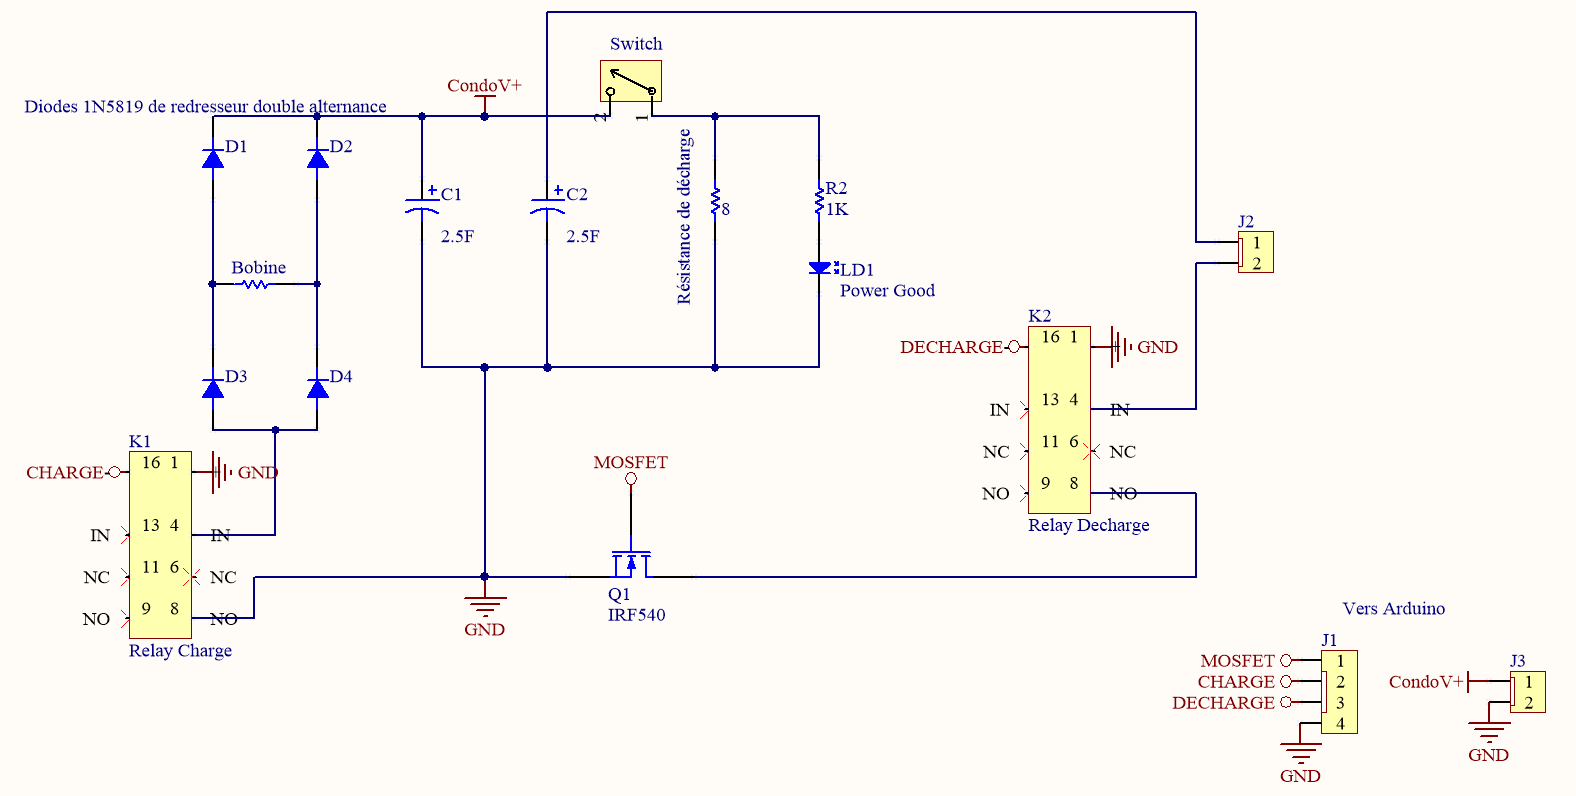
\includegraphics[width=1\textwidth]{fig/Condensateur.png}
   \caption{Sch�ma �lectrique de la charge et la d�charge du condensateur}
   \label{f:Condensateur}
\end{figure}



\section{Circuit de connections pour les moteurs}
\label{Connections}

\subsection{Connections moteurs et pont en H}
\label{Moteurs}

\begin{figure}[htp]
   \centering
   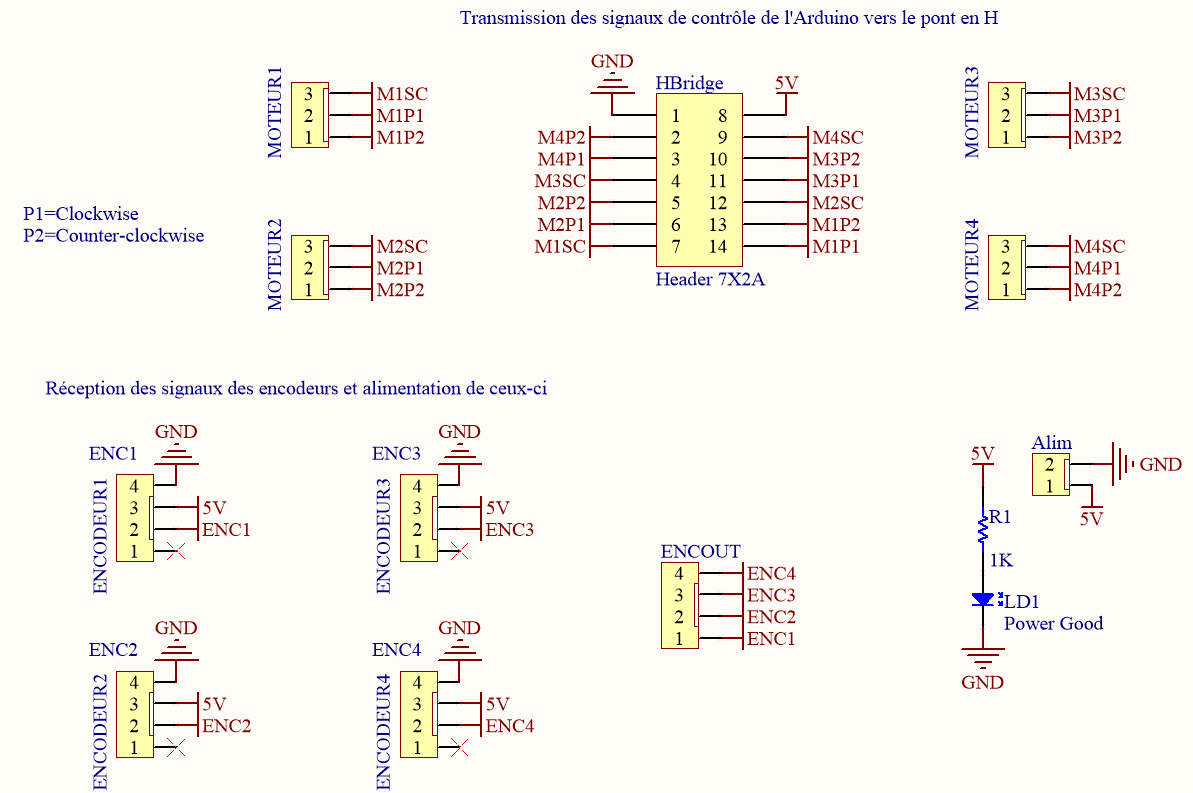
\includegraphics[width=1\textwidth]{fig/Connections.png}
   \caption{Sch�ma �lectrique du circuit de connections des moteurs}
   \label{f:Connections}
\end{figure}



\subsection{Connections sur l'Arduino}
\label{Arduino}




